\chapter{Pianificazione}\label{Pianificazione}
Jawa Druids ha deciso di pianificare il progetto in base alle scadenze riportate nel capitolo \ref{IntroduzioneScadenze}. Di conseguenza il progetto è stato suddiviso nelle seguenti fasi:
\begin{itemize}
	\item Analisi;
	\item Consolidamento dei requisiti;
	\item Progettazione architetturale;
	\item Progettazion di dettaglio e codifica;
	\item Validazione e collaudo.
\end{itemize}
Ognuna di queste fasi sarà formata da attività mostrate nei diagrammi di Gantt, che permettono la rappresentazione grafica di un calendario, utile al fine di pianificare, coordinare e tracciare specifiche attività in un progetto dando una chiara illustrazione del suo stato di avanzamento.
\section{Analisi}\label{PianificazioneAnalisi}
\textbf{Periodo:} dal 22-11-2020 al 11-01-2021
Questo periodo ha inizio con la formazione dei gruppi e termina con la scadenza per la consegna dei documenti relativi alla Revisione dei Requisiti.
Le principali attività svolte in questo periodo sono:
\begin{itemize}
	\item \textbf{Studio di Fattibilità:} attività nella quale viene effettuato uno studio di tutti i capitolati, elencando per ciascuno i punti positivi e negativi che li caratterizzano. Inoltre vengono indicate le motivazioni del perchè è stato scelto il capitolato GDP: Gathering Detection Platform e sono stati esclusi i rimanenti capitolati.
	Questa attività è bloccante per l'inizio dell'Analisi dei requisiti;
	\item \textbf{Norme di Progetto:} vengono definite tutte le regole, le convenzioni e le tecnologie che il gruppo Jawa Druids dovrà rispettare durante lo sviluppo dell'intero progetto;
	\item \textbf{Glossario:} racchiude termini che possono risultare ambigui durante lo svolgimento del progetto, e di essi viene fornita una breve descrizione;
	\item \textbf{Piano di Progetto:} il presente documento in cui le attività, i compiti, e le risorse precedentemente analizzate, vengono distribuite tra i membri del gruppo Jawa Druids. Inoltre presenta il calcolo del preventivo per la realizzazione del progetto e delle scadenze che il gruppo intende rispettare per la buona riuscita del progetto;
	\item \textbf{Lettera di Presentazione:} breve documento in cui il gruppo Jawa Druids si candida come fornitore del prodotto software richiesto;
	\item \textbf{Analisi dei requisiti:} vengono studiati e analizzati i requisiti del capitolato scelto nello Studio di Fattibilità;
	\item \textbf{Piano di qualifica:} attività nella quale gli Analisti redigono il Piano di Qualifica, documento in cui vengono indicate tutte le strategie di verifica e validazione che il gruppo intende adottare.
\end{itemize}
\subsection{Diagramma di Gantt:analisi}\label{PianificazioneDiagrammaDiGanttAnalisi}
\begin{figure}[!ht]
	\begin{center}
		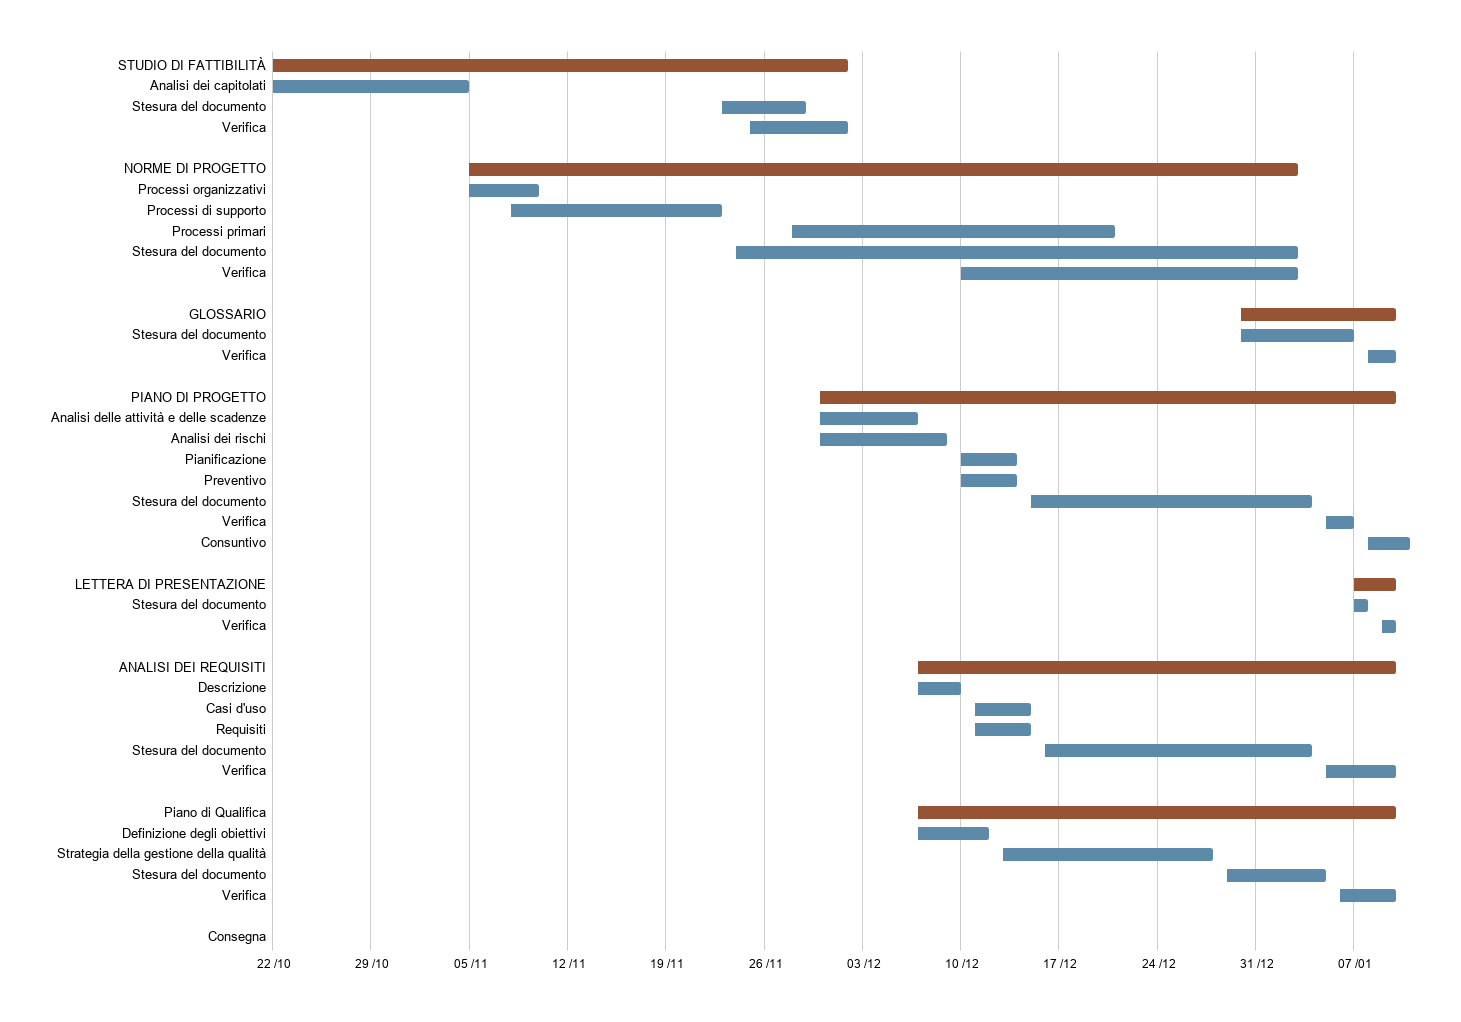
\includegraphics[width=1\linewidth]{../immagini/pdp/gantt_analisi.png}
		\caption{Diagramma di Gantt dell'attività di analisi}
	\end{center}
\end{figure}

\section{Conoslidamento dei requisiti}\label{PianificazioneConsolidamentoDeiRequisiti}
\textbf{Periodo:} dal 11-01-2021 al 18-01-2021
Questo periodo ha inizio subito dopo il termine del precedente e finisce con la presentazione della Revisione dei Requisiti.
Il gruppo Jawa Druids si dedicherà ai seguenti compiti:
\begin{itemize}
	\item avanzare con lo studio individuale relativo a:
	\begin{itemize}
		\item acquisizione dei dati;
		\item simulazione dei dati;
		\item machine learning;
		\item web app.
	\end{itemize}
	\item preparare il materiale necessario alla presentazione.
\end{itemize}
\subsection{Diagramma di Gantt consolidamento dei requisiti}\label{PianificazioneDiagrammaDiGanttConsolidamento}
\begin{figure}[!ht]
	\begin{center}
		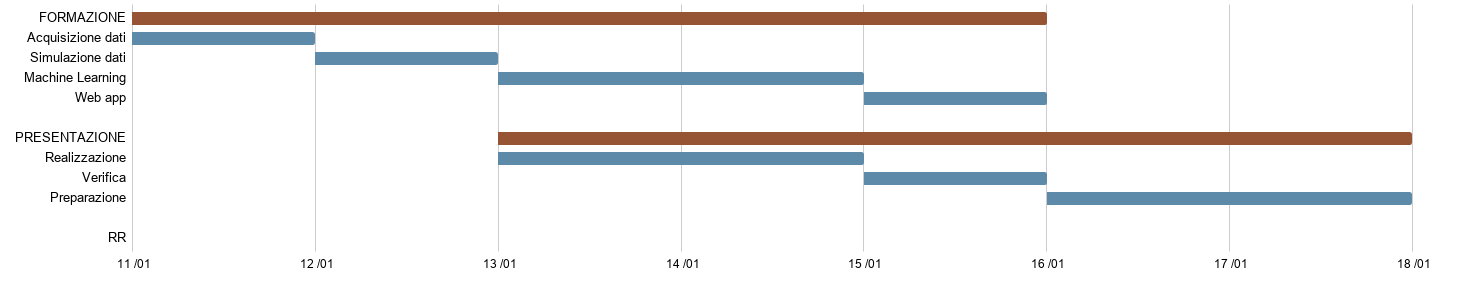
\includegraphics[width=1\linewidth]{../immagini/pdp/gantt_consolidamento_requisiti.png}
		\caption{Diagramma di Gantt del consolidamento dei requisiti}
	\end{center}
\end{figure}
\section{Progettazione architetturale}\label{PianificazioneProgettazioneArchitetturale}
\textbf{Periodo:} dal 18-01-2021 al 08-03-2021
Questo periodo ha inizio subito dopo essersi conclusa la precedente e termina con la Revisione di Progettazione.
Questo periodo porta all'individuazione di una soluzione architetturale che permetta il soddisfacimento dei requisiti individuali.
\begin{itemize}
	\item \textbf{Incremento e verifica:} come prima cosa, analizzando l'esito della Revisione dei Requisiti, vengono svolte attività di Incremento e Verifica sui vari documenti redatti, dove necessari.
	\item \textbf{Technology Baseline:} viene redatta la documentazione di supporto, contenente la descrizione delle tecnologie individuate e il tracciamento della relazione tra le componenti e i requisiti che vanno a soddisfare.
	Viene realizzato un Proof of Concept che verrà condiviso col proponente per verificare il corretto sviluppo del software.
\end{itemize}
\subsection{Diagramma di Gantt: progettazione architetturale}\label{PianificazioneDiagrammaDiGanttProgettazioneArchitetturale}
\begin{figure}[h]
	\begin{center}
		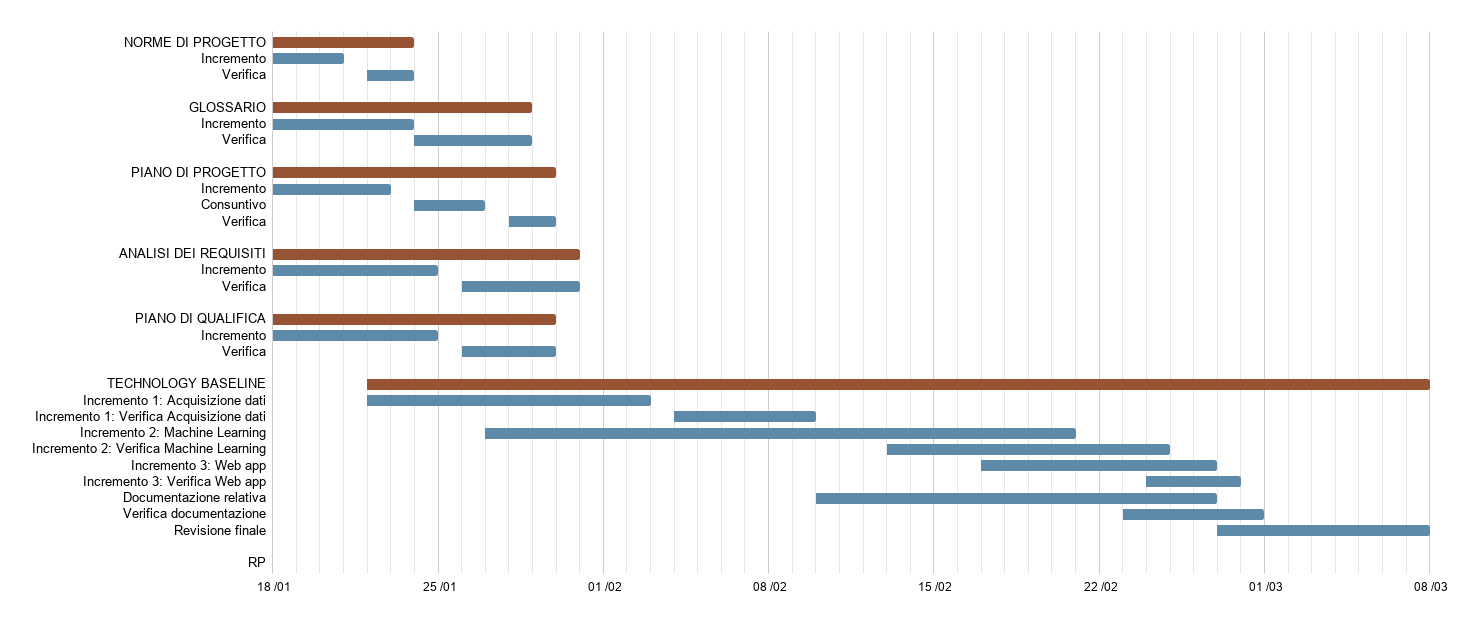
\includegraphics[width=0.9\linewidth]{../immagini/pdp/gantt_progettazione_architetturale.png}
		\caption{Diagramma di Gantt della progettazione architetturale}
	\end{center}
\end{figure}
\section{Progettazione di dettaglio e codifica}\label{PianificazioneProgettazioneDettaglio}
\textbf{Periodo:} dal 15-03-2021 al 09-04-2021
Questo periodo inizia appena conclusa la precedente e termina con la Revisione di Qualifica.
Le principali attività svolte in questo periodo sono
\begin{itemize}
	\item \textbf{Incremento e verifica:} alcuni dei documenti già prodotti vengono migliorati e aggiornati;
	\item \textbf{Product Baseline:} segue la Technology Baseline, dove vengono studiati meglio design, pattern, classi e attività necessarie alla codifica;
	\item \textbf{Specifica Tecnica:} è un documento contenente tutte le caratteristiche del prodotto e le motivazioni che hanno portato alla loro scelta;
	\item \textbf{Codifica:} attività nella quale viene prodotto e verificato il codice;
	\item \textbf{Manuale utente:} attività nella quale viene redatto il documento contenente le informazioni su come funziona e su come si utilizza il prodotto.
\end{itemize}
\subsection{Diagramma di Gantt: progettazione di dettaglio e codifica}\label{PianificazioneDiagrammaDiGanttProgettazioneDettaglio}
\begin{figure}[!ht]
	\begin{center}
		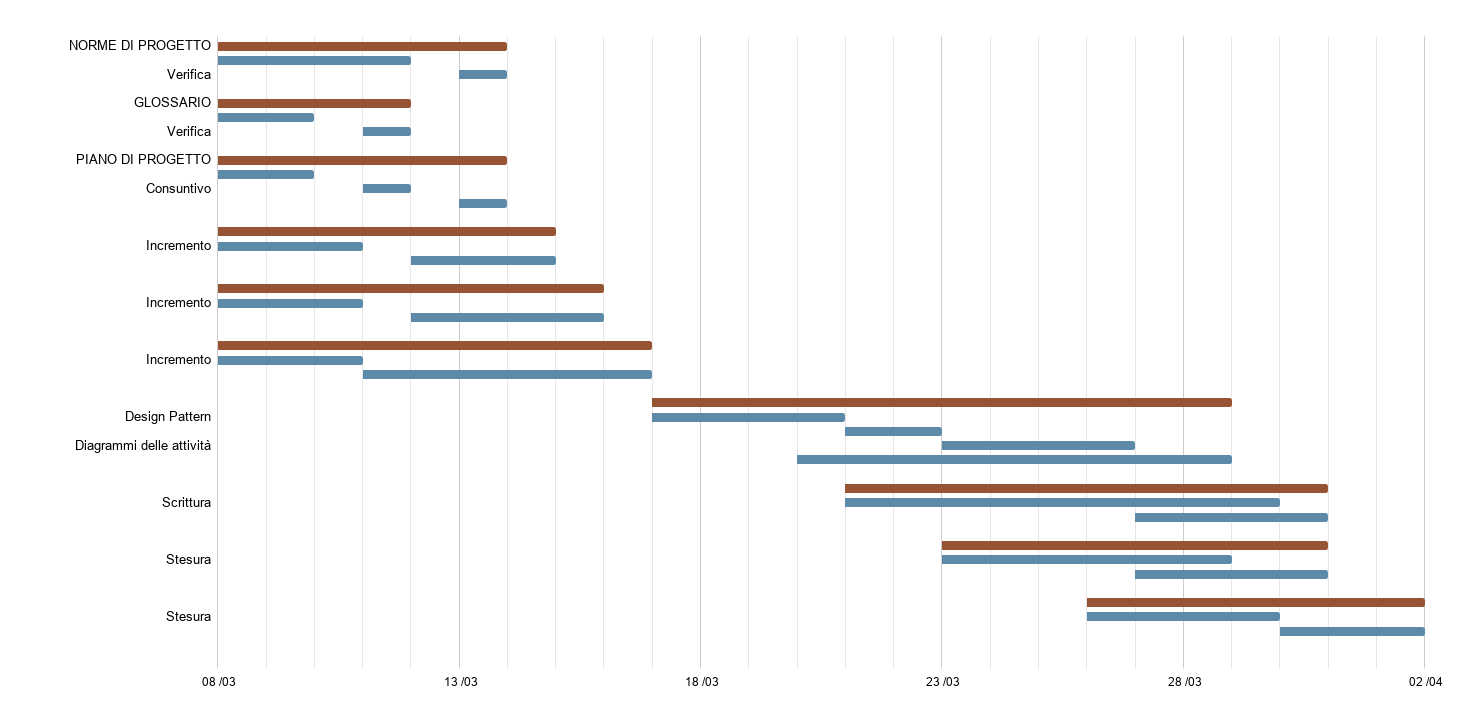
\includegraphics[width=0.8\linewidth]{../immagini/pdp/gantt_progettazione_dettaglio.png}
		\caption{Diagramma di Gantt dell'attività di progettazione di dettaglio e codifica}
	\end{center}
\end{figure}
\section{Validazione e Collaudo}\label{PianificazioneValidazione}
\textbf{Periodo:} dal 16-04-2021 al 10-05-2021
Questo periodo inizia appena conclusa la precedente e termina con la Revisione di Accettazione.
Le principali attività svolte in questo periodo sono
\begin{itemize}
	\item \textbf{Incremento e verifica:} come prima cosa, analizzando l'esito della Revisione di Qualifica vengono svolte attività di Incremento e Verifica sui vari documenti redatti;
	\item \textbf{Validazione e Collaudo:} vengono realizzati gli ultimi test, con i dovuti controlli finali in modo da garantire un buon livello di qualità e correttezza.
\end{itemize}
\subsection{Diagramma di Gantt: validazione e collaudo}\label{PianificazioneDiagrammaDiGanttValidazione}
\begin{figure}[!ht]
	\begin{center}
		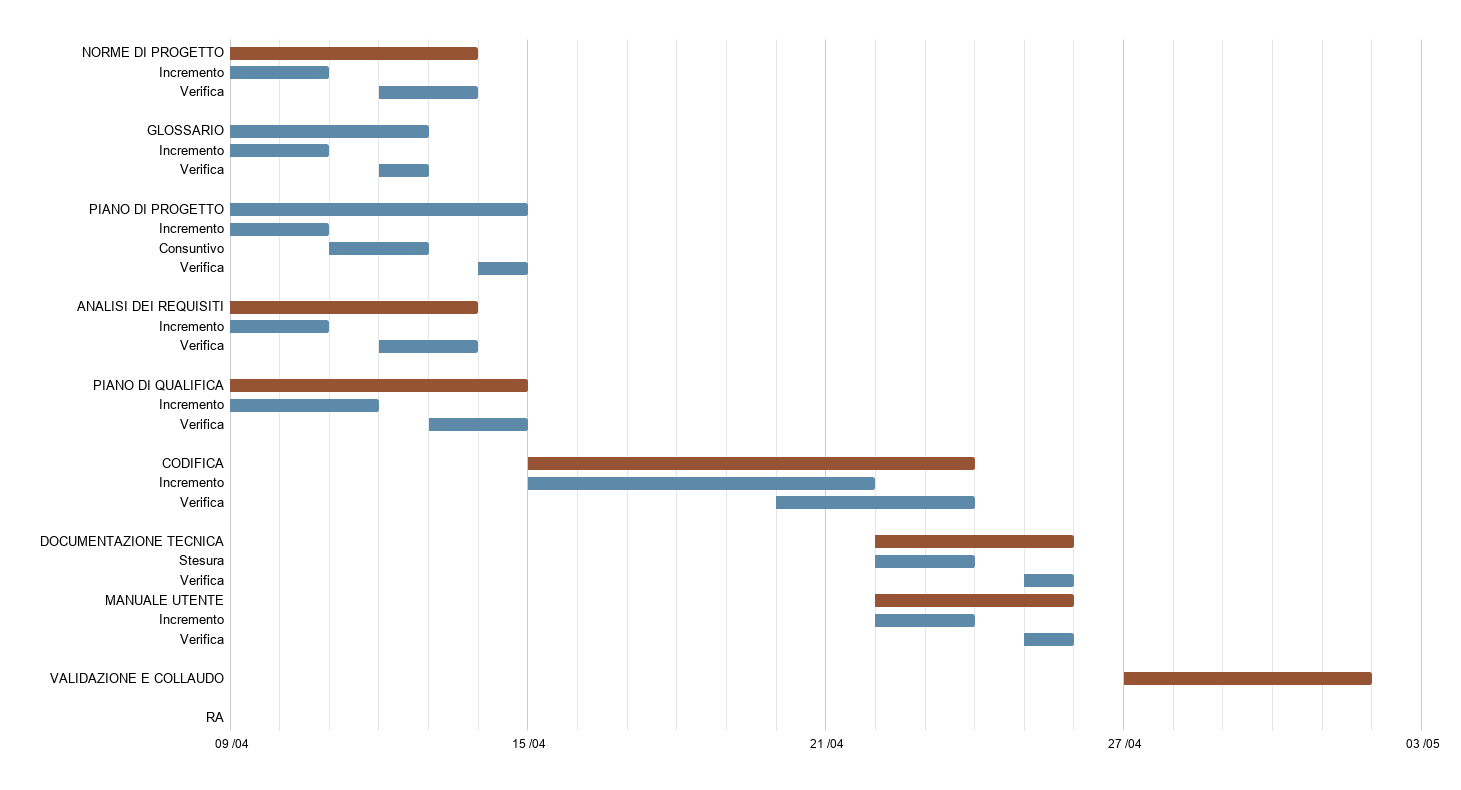
\includegraphics[width=0.8\linewidth]{../immagini/pdp/gantt_validazione.png}
		\caption{Diagramma di Gantt dell'attività di validazione e collaudo}
	\end{center}
\end{figure}